% =====================================================================
% Rozdział 3 – Projekt systemu (~9 str.)
% Z czego i jak zbudowany system, dlaczego tak. Bez powtarzania teorii.
% =====================================================================
\chapter{Projekt systemu}
\label{ch:projekt}
W~rozdziale przedstawiono projekt systemu, czyli jego budowę sprzętową
i~decyzje podjęte przed implementacją. Na początku określono wymagania
stawiane systemowi oraz jego ogólną koncepcję, w~tym podział zadań między
węzły kamerowe a~komputer nadrzędny (podrozdz.~\ref{sec:wymagania}).
Następnie opisano węzeł kamerowy wraz z~uzasadnieniem wyboru mikrokontrolera
i~modułu kamery (podrozdz.~\ref{sec:wezel}) oraz rozmieszczenie kamer
zapewniające pokrycie pełnego kąta wokół robota (podrozdz.~\ref{sec:rozmieszczenie}).
W~dalszej części przedstawiono obudowę systemu i~sposób jej montażu na
robocie JetBot (podrozdz.~\ref{sec:obudowa}), a~na końcu komputer nadrzędny
oraz sieć łączącą go z~węzłami (podrozdz.~\ref{sec:komputer-siec}).
Implementację oprogramowania, kalibracji i~fuzji danych opisano
w~rozdziale~\ref{ch:implementacja}.
% ---------------------------------------------------------------------
\section{Wymagania i~koncepcja systemu}
\label{sec:wymagania}
% - Wymagania funkcjonalne: wykrywanie obiektów dookoła robota,
%   wyznaczenie kierunku, publikacja w ROS 2, kalibracja.
% - Wymagania niefunkcjonalne: ok. 5–10 FPS na kamerę, opóźnienie rzędu
%   kilkuset ms lub mniej, niski koszt, skalowalność liczby kamer.
% - Uzasadnienie głównych wyborów: FOMO zamiast SSD/YOLO, int8,
%   kalibracja szachownicą i korekcja dystorsji, fuzja na komputerze,
%   UDP zamiast TCP.
% - Koncepcja: 6 węzłów (ESP32-S3 + kamera + FOMO) -> Wi-Fi/UDP ->
%   komputer nadrzędny (odbiór, fuzja) -> ROS 2.
% - Podział obowiązków: węzeł = obraz -> detekcja; komputer =
%   synchronizacja, fuzja, publikacja.
% - Przepływ danych: klatka 320x240 -> LUT -> 96x96 -> FOMO -> centroid
%   -> pakiet UDP -> odbiór -> azymut -> fuzja -> komunikat ROS 2.
% - Rys.: schemat blokowy systemu (schemat_systemu.drawio).
% - Rys.: przepływ danych w węźle i na komputerze.
% Stan: ✅ tekst; ⏳ rys. przepływu danych (imgs/przeplyw_danych.drawio.png),
%       ⏳ sprawdzić etykiety \ref do rozdz. 2, 3 i 4.

Celem projektowanego systemu jest dostarczenie robotowi mobilnemu
informacji o~otaczających go obiektach, niezależnie od kierunku,
w~którym się znajdują. Przed przystąpieniem do projektowania należało
sformułować wymagania, a~następnie na ich podstawie opracować koncepcję
działania systemu.

\subsubsection*{Wymagania funkcjonalne}

\begin{itemize}[nosep]
  \item System wykrywa obiekty zadanej klasy w~pełnym zakresie
        $360^\circ$ wokół robota.
  \item Dla każdego wykrytego obiektu wyznaczany jest jego kierunek
        (azymut) w~układzie współrzędnych robota, klasa oraz pewność
        detekcji.
  \item Detekcje pochodzące z~różnych kamer, dotyczące tego samego
        obiektu, są łączone w~jeden wynik.
  \item Każda detekcja opatrzona jest znacznikiem czasu odpowiadającym
        chwili wykonania zdjęcia.
  \item Wyniki są publikowane w~środowisku ROS~2, co umożliwia ich
        wykorzystanie przez pozostałe moduły oprogramowania robota.
  \item System umożliwia przeprowadzenie kalibracji kamer oraz
        wyznaczenie ich położenia i~orientacji na robocie.
\end{itemize}

\subsubsection*{Wymagania niefunkcjonalne}

\begin{itemize}[nosep]
  \item Praca w~czasie rzeczywistym: częstotliwość detekcji na poziomie
        5--10~klatek na sekundę dla każdej kamery.
  \item Opóźnienie od wykonania zdjęcia do udostępnienia wyniku rzędu
        kilkuset milisekund lub mniejsze.
  \item Błąd wyznaczenia azymutu rzędu kilku stopni.
  \item Niski koszt pojedynczego węzła kamerowego oraz możliwość łatwej
        zmiany liczby kamer.
  \item Minimalne obciążenie komputera nadrzędnego i~sieci.
  \item Bezprzewodowa komunikacja węzłów z~komputerem nadrzędnym.
  \item Odporność na awarie: utrata pojedynczych pakietów lub wyłączenie
        jednego węzła nie zatrzymuje pracy pozostałej części systemu.
  \item Możliwość montażu na robocie JetBot -- ograniczone wymiary
        konstrukcji oraz zasilanie węzłów z~płytki robota.
\end{itemize}

\subsubsection*{Koncepcja systemu}

Na podstawie powyższych wymagań przyjęto architekturę rozproszoną,
w~której przetwarzanie obrazu odbywa się bezpośrednio na węzłach
kamerowych, a~komputer nadrzędny otrzymuje jedynie wyniki detekcji
zamiast strumienia obrazu. Schemat blokowy systemu przedstawiono na
rys.~\ref{fig:schemat-systemu}.

\begin{figure}[htbp]
  \centering
  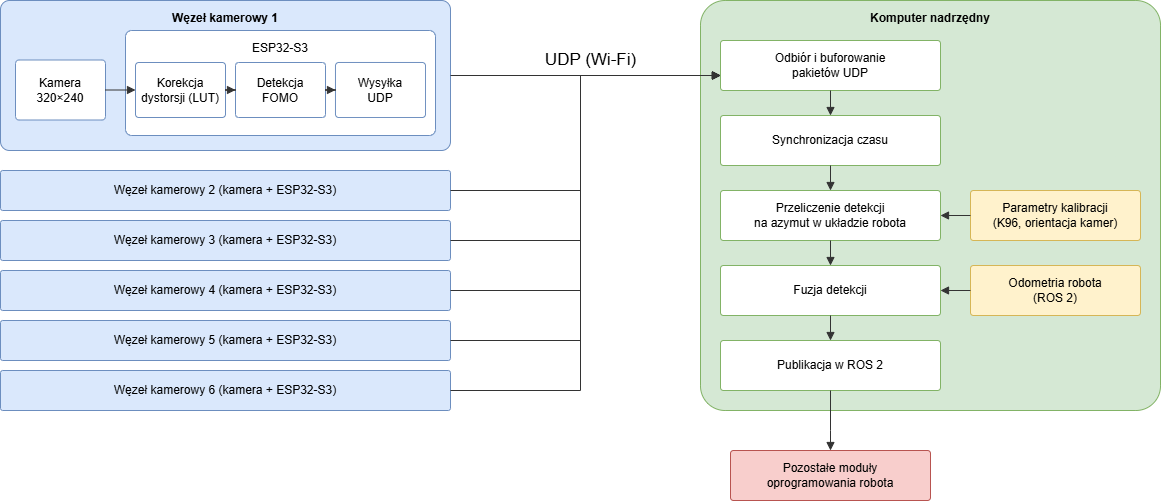
\includegraphics[width=\textwidth]{imgs/schemat_systemu.drawio.png}
  \caption{Schemat blokowy systemu. Przetwarzanie obrazu odbywa się na
    węzłach kamerowych, a~do komputera nadrzędnego trafiają jedynie
    wyniki detekcji}
  \label{fig:schemat-systemu}
\end{figure}

System składa się z~sześciu węzłów kamerowych rozmieszczonych dookoła
robota co $60^\circ$ oraz komputera nadrzędnego. Każdy węzeł zbudowany
jest z~mikrokontrolera ESP32-S3 i~modułu kamery. Węzły komunikują się
z~komputerem przez sieć Wi-Fi z~wykorzystaniem protokołu UDP. Obowiązki
poszczególnych elementów podzielono następująco:

\begin{itemize}[nosep]
  \item \textbf{węzeł kamerowy} -- akwizycja obrazu, korekcja dystorsji,
        inferencja modelu detekcji oraz wysłanie wyniku,
  \item \textbf{komputer nadrzędny} -- odbiór danych ze wszystkich
        węzłów, synchronizacja czasowa, przeliczenie detekcji do układu
        robota, fuzja oraz publikacja wyników w~ROS~2.
\end{itemize}

Taki podział wynika z~dysproporcji zasobów: mikrokontroler jest w~stanie
wykonać inferencję niewielkiej sieci neuronowej, natomiast operacje
wymagające danych ze wszystkich kamer jednocześnie oraz integracja
z~ROS~2 realizowane są na komputerze. Dzięki temu na węzłach nie jest
potrzebne środowisko micro-ROS (odmiana ROS~2 przeznaczona dla
mikrokontrolerów, wymagająca dodatkowego agenta uruchomionego na
komputerze), a~rozmiar przesyłanych danych ogranicza się do
kilkudziesięciu bajtów na klatkę.

\subsubsection*{Przepływ danych}

Przepływ danych w~węźle kamerowym i~na komputerze nadrzędnym
przedstawiono na rys.~\ref{fig:przeplyw-danych}. Węzeł pobiera
z~kamery klatkę o~rozdzielczości $320\times240$ pikseli w~odcieniach
szarości. Za pomocą tablicy przekodowań LUT (ang.~\textit{Look-Up
Table}) obraz jest jednocześnie korygowany z~dystorsji i~skalowany do
rozmiaru wejścia modelu, czyli $96\times96$ pikseli. Model FOMO zwraca
centroidy wykrytych obiektów wraz z~klasą i~pewnością. Wyniki, razem
ze znacznikiem czasu wykonania zdjęcia, są wysyłane w~pakiecie UDP.
Komputer nadrzędny odbiera pakiety, przelicza położenie centroidu na
azymut w~układzie robota, łączy detekcje pochodzące z~różnych kamer
i~publikuje wynik jako komunikat ROS~2.

\begin{figure}[htbp]
  \centering
  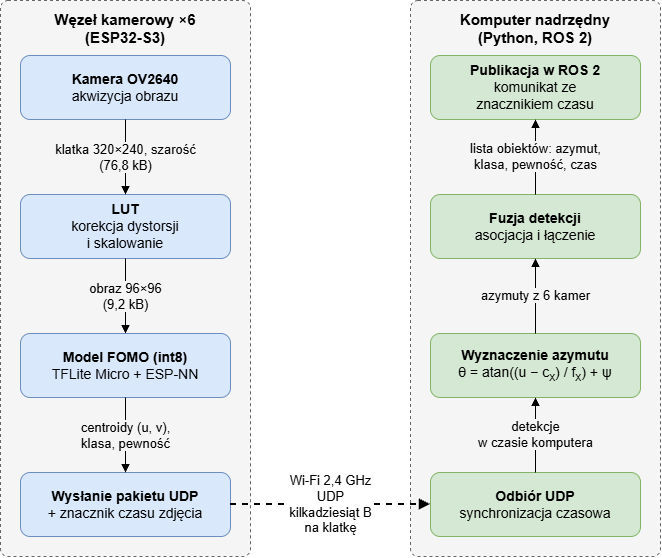
\includegraphics[width=\textwidth]{imgs/przeplyw_danych.drawio.png}
  \caption{Przepływ danych w~węźle kamerowym i~na komputerze nadrzędnym.
    Obraz nie opuszcza węzła -- przez sieć przesyłane są jedynie
    centroidy wykrytych obiektów}
  \label{fig:przeplyw-danych}
\end{figure}

\subsubsection*{Uzasadnienie przyjętych rozwiązań}

Na podstawie przeglądu przedstawionego w~rozdz.~\ref{ch:teoria}
przyjęto następujące rozwiązania:

\begin{itemize}[nosep]
  \item \textbf{FOMO zamiast detektorów SSD i~YOLO} -- do wyznaczenia
        kierunku wystarczy położenie środka obiektu. FOMO zwraca
        centroidy i~mieści się w~pamięci mikrokontrolera, natomiast
        detektory zwracające prostokąty wymagają wielokrotnie więcej
        pamięci i~obliczeń (podrozdz.~\ref{sec:detekcja-mcu}).
  \item \textbf{Kwantyzacja int8} -- czterokrotnie mniejszy model
        i~arytmetyka całkowita z~użyciem instrukcji SIMD, kosztem
        niewielkiego spadku dokładności.
  \item \textbf{Kalibracja szachownicą i~korekcja dystorsji na węźle} --
        model otrzymuje obraz bez zniekształceń, spójny dla wszystkich
        kamer, a~kierunek do obiektu można wyznaczyć z~modelu
        otworkowego (podrozdz.~\ref{sec:model-kamery}).
  \item \textbf{UDP zamiast TCP} -- nieaktualny wynik detekcji nie ma
        wartości, więc utrata pojedynczego pakietu jest mniej szkodliwa
        niż opóźnienie wynikające z~retransmisji
        (podrozdz.~\ref{sec:protokoly}).
\end{itemize}

Dobór sprzętu węzła kamerowego opisano w~podrozdz.~\ref{sec:wezel},
rozmieszczenie kamer w~podrozdz.~\ref{sec:rozmieszczenie}, obudowę
w~podrozdz.~\ref{sec:obudowa}, a~komputer nadrzędny i~sieć
w~podrozdz.~\ref{sec:komputer-siec}. Implementację poszczególnych
elementów przedstawiono w~rozdz.~\ref{ch:implementacja}.


% ---------------------------------------------------------------------
\section{Węzeł kamerowy}
\label{sec:wezel}
% - ESP32-S3: 2 rdzenie Xtensa LX7 240 MHz, ok. 512 kB SRAM, PSRAM 8 MB
%   octal 80 MHz, SIMD (ESP-NN), interfejs kamery DVP, Wi-Fi 2,4 GHz.
%   ⏳ sprawdzić liczby w datasheecie.
% - Punkt wyjścia: ESP32-CAM (AI-Thinker, ESP32-D0WD-V3, LX6, OV3660) –
%   pierwsze zdjęcia i pierwsze wersje.
% - Dlaczego S3: za mało RAM wewnętrznego i wolniejsza PSRAM na ESP32,
%   brak SIMD -> ESP-NN nie przyspiesza; S3 mieści arenę modelu (270 kB)
%   i bufory kamery.
% - Tab.: ESP32 vs ESP32-S3 (rdzenie, taktowanie, SRAM, PSRAM, SIMD,
%   ESP-NN, USB, cena).
% - Kamera: sensor (OV2640 na płytce S3, wcześniej OV3660), QVGA 320x240,
%   odcienie szarości, XCLK.
% - Wybór kąta widzenia: mniejszy FOV (mniejsza dystorsja, więcej pikseli
%   na obiekt, ale 6 kamer nie pokryje 360°) vs większy FOV (pokrycie
%   z nakładaniem, większa dystorsja); wymaganie 70–90°, wybrano HFOV 76°.
%   Rzeczywisty HFOV z kalibracji vs deklaracja producenta. ⏳
% - Tab.: porównanie rozważanych modułów kamer (sensor, FOV, dystorsja,
%   dostępność).
% - Płytka: GOOUUU ESP32-S3-CAM (N16R8: 16 MB flash, 8 MB PSRAM) –
%   złącza, programowanie przez USB.
% - Wzmianka: rozważano własną płytkę węzła (PCB), zrezygnowano –
%   1–2 zdania dlaczego (czas, koszt, gotowe moduły wystarczają).
% - Pobór prądu węzła (średni i szczytowy przy nadawaniu Wi-Fi). ⏳
% - Rys.: zdjęcie węzła.
% Stan: ✅ / ⏳


% ---------------------------------------------------------------------
\section{Rozmieszczenie kamer}
\label{sec:rozmieszczenie}
% - Geometria: 6 kamer co 60° na ściankach sześciokąta foremnego.
% - Minimalny HFOV dla pokrycia 360°: 360°/6 = 60°.
% - Nakładanie przy HFOV 76°: ok. 16° na każdą parę sąsiednich kamer –
%   potrzebne do fuzji i niezawodności.
% - Martwe strefy blisko robota (kamery nie są w jednym punkcie) –
%   odległość, od której pokrycie jest pełne.
% - Rozdzielczość kątowa FOMO: 12 komórek w poziomie ->
%   komórka ≈ 76°/12 ≈ 6,3°.
% - Wysokość montażu i pochylenie kamer – widoczny zakres odległości
%   i wysokości obiektów.
% - Rys.: widok z góry – robot, 6 kamer, pola widzenia, obszary nakładania.
% Stan: ⏳ (martwe strefy, wysokość)




% ---------------------------------------------------------------------
\section{Obudowa i~montaż na robocie JetBot}
\label{sec:obudowa}
% - Platforma: JetBot ROS AI Kit; zdemontowana przednia kamera robota.
%   Obudowa zaprojektowana na podstawie modelu STEP robota.
% - Forma: nakładka Ø200 mm z wcięciami na koła.
% - Kamery: 6 osobnych modułów (korpus 14x14 mm z uszami na śruby)
%   na ściankach sześciokąta foremnego – zgodnie z \ref{sec:rozmieszczenie}.
% - Węzły: 6x ESP32-S3 pionowo we wsuwanych slotach.
% - Zasilanie: po goldpinach z PCB robota; środek nakładki otwarty nad
%   płytką robota. Rozprowadzenie zasilania 6 węzłów i bilans prądowy
%   względem możliwości robota. ⏳
% - Ograniczenia konstrukcyjne: strefa przy 2 antenach robota (przy
%   wcięciach kół) pusta; chłodzenie tylko pasywne (szczeliny,
%   bez wentylatorów).
% - Wykonanie: model parametryczny w OpenSCAD, druk 3D (parametry druku,
%   materiał – jeśli dostępne). ⏳
% - Rys.: render/rzut obudowy z polami widzenia.
% - Rys.: zdjęcie systemu zamontowanego na robocie.
% Stan: ✅ (projekt) / ⏳ (wydruk, zdjęcia, zasilanie)


% ---------------------------------------------------------------------
\section{Komputer nadrzędny i~sieć}
\label{sec:komputer-siec}
% - Komputer: PC AMD Ryzen 5 3600, 16 GB RAM, Windows 11 Pro – odbiór UDP,
%   fuzja, ROS 2. ⏳ wersja ROS 2 i sposób uruchomienia na Windows.
% - Sieć: węzły i komputer w lokalnej sieci Wi-Fi 2,4 GHz (wspólny
%   router) – sprawdzić zgodność ze schematem blokowym; adresacja
%   (statyczne IP / DHCP), port UDP. ⏳
% - Przepustowość: pakiety po kilkadziesiąt bajtów, ok. 9 Hz x 6 węzłów –
%   sieć nie jest wąskim gardłem; porównanie z wysyłaniem obrazu.
% - Rys.: topologia sieci.
% Stan: ⏳
Odbiór danych z~węzłów, fuzja detekcji oraz publikacja wyników w~ROS~2
realizowane są na komputerze nadrzędnym. Zastosowano komputer stacjonarny
z~procesorem AMD Ryzen~5 3600 (6~rdzeni, 12~wątków, taktowanie bazowe
3,6~GHz) i~16~GB pamięci RAM, pracujący pod kontrolą systemu Windows~11.
[ TODO - sprawdzić wersje ]Środowisko ROS~2 (dystrybucja \textit{Humble}) uruchomiono w~podsystemie
WSL~2 (ang.~\textit{Windows Subsystem for Linux}) z~systemem Ubuntu~22.04.
Obciążenie obliczeniowe komputera jest niewielkie, ponieważ nie przetwarza
on obrazu, a~jedynie kilka detekcji na klatkę z~każdej kamery.
W~szczególności nie jest wykorzystywana karta graficzna -- cała inferencja
sieci neuronowej odbywa się na węzłach.

Każdy z węzłów przesyła wyniki detekcji do komputera nadrzędnego
z wykorzystaniem protokołu UDP. Węzły i komputer pracują w tej samej
lokalnej sieci, zbudowanej na typowym domowym routerze. Węzły łączą się
z punktem dostępowym routera przez Wi-Fi w paśmie 2,4~GHz (moduł ESP32-S3
obsługuje tylko to pasmo), natomiast komputer jest dołączony do routera
przez Wi-Fi. Adresy IP przydziela
wszystkim urządzeniom serwer DHCP routera. Adres komputera nadrzędnego
i numer portu docelowego (5005) zapisano w konfiguracji oprogramowania
węzłów. Na komputerze program odbiorczy nasłuchuje na tym porcie na
wszystkich interfejsach sieciowych. Nadawcę pakietu rozpoznaje po polu
identyfikatora kamery, a nie po adresie IP. Dzięki temu zmiana adresów
węzłów przy ponownym przydziale DHCP nie wpływa na działanie systemu.

Ilość przesyłanych danych jest bardzo mała. Pojedynczy pakiet zawiera
identyfikator węzła, klasę, współrzędne centroidu, pewność detekcji oraz
znacznik czasu (podrozdział~\ref{sec:protokoly}). Przyjmując rozmiar
pakietu wraz z nagłówkami rzędu 60~B, sześć węzłów pracujących
z częstotliwością ok. 9 klatek na sekundę generuje strumień ok.
$6 \cdot 9 \cdot 60\,\mathrm{B} \approx 3{,}2$~kB/s.
% TODO: podstawić rzeczywisty rozmiar pakietu
Dla porównania przesyłanie surowych klatek QVGA w odcieniach szarości
($320 \cdot 240 = 76{,}8$~kB na klatkę) z tą samą częstotliwością
wymagałoby przepustowości ok. 4,1~MB/s, czyli ok. 33~Mbit/s, co w sieci
Wi-Fi współdzielonej przez sześć urządzeń prowadziłoby do znacznych
opóźnień i utraty danych. Przetwarzanie obrazu na węzłach sprawia więc, że
sieć nie stanowi wąskiego gardła systemu.


